To perform an end-to-end evaluation on our prototype,
we layered our mi

\textbf{Metadata Intensive Workloads}

\begin{figure}[t]  %%%%%%%%%%%%%%%%%%%%%%%
\centerline{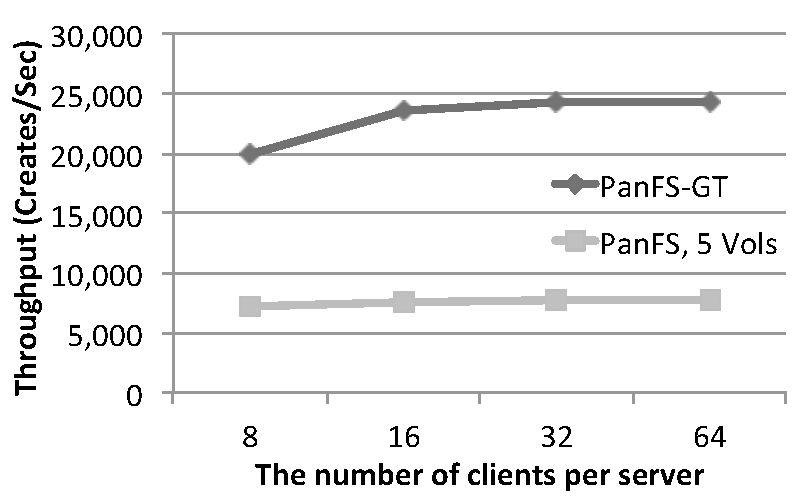
\includegraphics[scale=0.5]{./figs/zero_file_creation_on_panfs}}
\vspace{10pt}
\caption{\normalsize
Create five million zero-length files in one empty directory
with different number of clients.
\textit{}
}
\vspace{10pt}
\hrule
\label{graph:ldb-singlenode}
\end{figure}       %%%%%%%%%%%%%%%%%%%%%%%

\begin{figure}[t]  %%%%%%%%%%%%%%%%%%%%%%%
\centerline{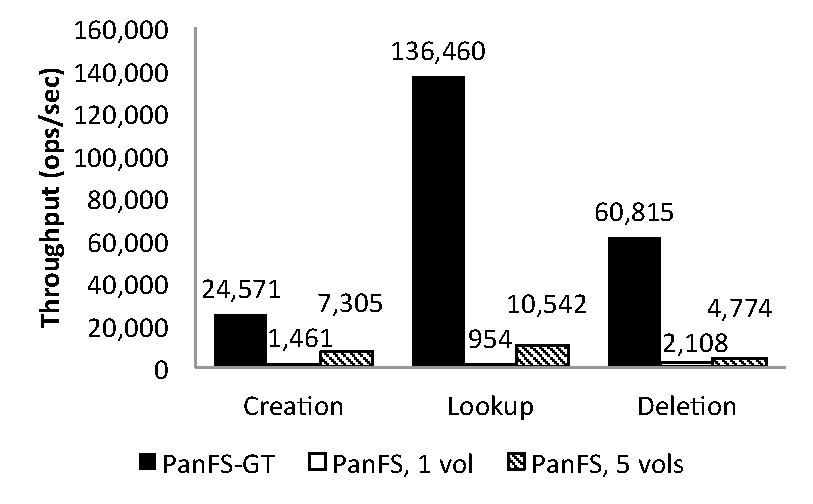
\includegraphics[scale=0.6]{./figs/mdtest}}
\vspace{10pt}
\caption{\normalsize
\textit{mdtest:
Create 5 million zero-length files in one shared directory.
}
}
\vspace{10pt}
\hrule
\label{graph:ldb-singlenode}
\end{figure}       %%%%%%%%%%%%%%%%%%%%%%%


\begin{figure}[t]  %%%%%%%%%%%%%%%%%%%%%%%
\centerline{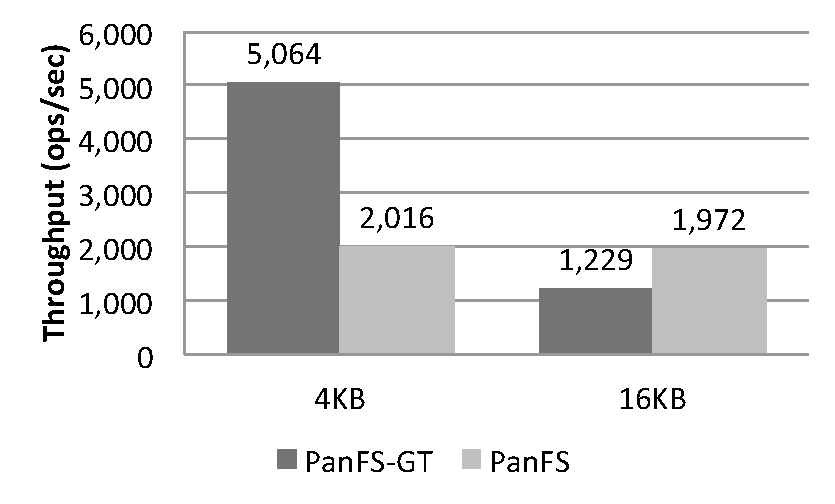
\includegraphics[scale=0.5]{./figs/small_file_creates}}
\vspace{10pt}
\caption{\normalsize
\textit{Create 5 million small files with different size
in one share directory}
}
\vspace{10pt}
\hrule
\label{graph:ldb-singlenode}
\end{figure}       %%%%%%%%%%%%%%%%%%%%%%%

\begin{figure}[t]  %%%%%%%%%%%%%%%%%%%%%%%
\centerline{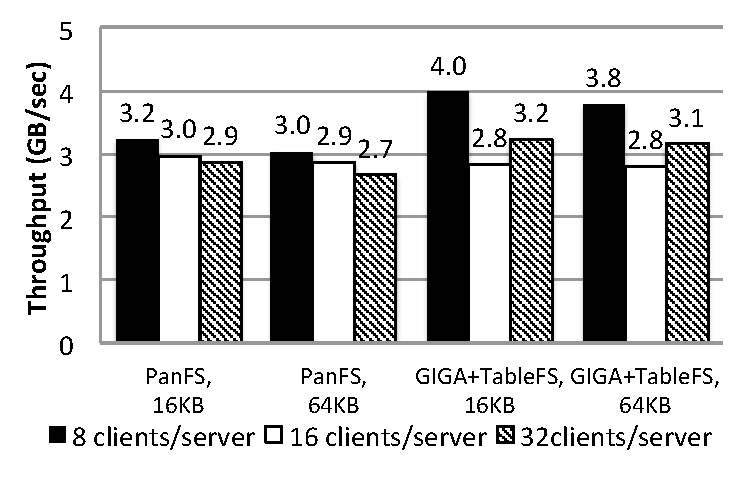
\includegraphics[scale=0.6]{./figs/checkpointing_write}}
\vspace{10pt}
\caption{\normalsize
\textit{
The aggregated write throughput in N-N check-pointing workload.
Each volume receives 640 GB data.
}
}
\vspace{10pt}
\hrule
\label{graph:ldb-singlenode}
\end{figure}       %%%%%%%%%%%%%%%%%%%%%%%

\begin{figure}[t]  %%%%%%%%%%%%%%%%%%%%%%%
\centerline{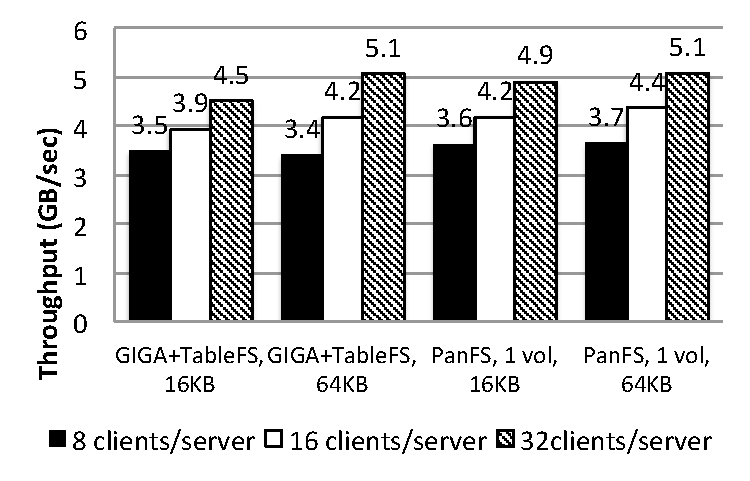
\includegraphics[scale=0.6]{./figs/checkpointing_read}}
\vspace{10pt}
\caption{\normalsize
\textit{
The aggregated read throughput in N-N check-pointing workload.
}
}
\vspace{10pt}
\hrule
\label{graph:ldb-singlenode}
\end{figure}       %%%%%%%%%%%%%%%%%%%%%%%

